   \chapter{Background}
\label{chap:background}

In this chapter, we present the fundamental concepts and technologies relevant
to this work. These background elements provide the
necessary context for understanding the datasets, preprocessing
pipeline, and anomaly detection approaches presented in the
subsequent chapters.


\section{Machine Learning Terminology}
\subsection{Machine learning}
Machine learning is an evolving branch of computational algorithms that are designed to emulate human intelligence by learning from the surrounding environment. They are considered the working horse in the new era of the so-called big data. Techniques based on machine learning have been applied successfully in diverse fields ranging from pattern recognition, computer vision, spacecraft engineering, finance, entertainment, and computational biology to biomedical and medical applications. These methods can help us in creating anomaly detection systems which are able to detect outliers, or classify new network packets as malicious. Usually machine learning is split into two major methods which are \textit{Supervised learning} and \textit{Unsupervised learning}. In machine learning we usually consider set of objects O which is divided into previously seen data S, and previously unseen data U, and the goal is to build a mathematical model M - which can be seen as mapping function which converts the input into certain output - that can learn from S, and apply its knowledge on U with generalization to get the best results. 
\subsection{Overfitting}
This is a phenomenon happens when the model performs very good during the training phase, but the performance drops significantly during testing phase. Usually this means that the model can not generalize to previously unseen data, and it just memorizes the training data. We will sometimes refer to this concept when we obtain very high results on our metrics, and we try to generally avoid it.  
\subsection{Underfitting}
This is a phenomenon happens when the model performs poorly during both training and testing phases. Usually this means that the underlying function is much more complex than the ability of the model to learn. This usually means that the model has high bias and that the underlying mathematical function is more complex than our model.
\subsection{Supervised learning}
It is a method from machine learning, where we already have previously seen data S, with their corresponding labels, and we try to teach our model M based on these previous labels, in order to be able to predict the labels of U correctly. Examples are classification and regression. 
\subsection{Unsupervised learning}
This is another method from machine learning, where there are no labels for the training data, instead the model try to learn patterns and relations between the data. Examples are outlier detection and clustering. 
\subsection{Distance functions}
Usually when we are working in any feature space, we need to measure the distance between two points in this space. In order to do so, we need to define a distance function that can evaluate these distances. There are some famous distance functions such as the Manhattan ($L_1$) distance function, which computes the distance as the summation of the absolute difference between each feature for two different points. It can be seen as follows: for $p,q \in \mathbb{R}^n$, $\|dist(p,q)\|_1 = \sum_{i=1}^{n} |p_i - q_i|$. Another famous distance function is the Euclidean distance ($L_2$), which computes the square root of the sum of the squared differences between feature values. It can be seen as follows: for $p,q \in \mathbb{R}^n$, $\|dist(p,q)\|_2 = \sqrt{\sum_{i=1}^{n} (p_i - q_i)^2}$.
\subsection{Levels of measurements for features}
We can categorize data types into three major types. Firstly, \textit{Nominal} data which are categorical, where we only ascertain whether value exist or not i.e. boolean, and there is no order for such data, and we can not also define distance function for them. Secondly, ordinal data where there exist an order relation (better/worse) between categories, but no uniform distance i.e. University grades (A+, B-, etc...). Finally, metric which can  both differences and ratios between the values are meaningful. The values can be discrete or continuous. i.e. weight (continuous), age classes (discrete). In our evaluation, we will use the latter level. Specifically, we will use precision, recall, and F1-score to evaluate our models' performance.
 
\subsection{K-Folding}
The dataset is divided into $k$ equally sized folds.
In each iteration, one fold is used as the validation (test) split,
while the remaining $k-1$ folds form the training split.
This process is repeated $k$ times such that each fold serves once
as validation data. Final performance metrics are obtained by
averaging over all $k$ runs.  

\subsection{F1-Score}
In binary classification, the performance of a model can be evaluated using the metrics precision, recall, and F1-score. Let $TP$ denote the number of true positives, $FP$ the number of false positives, and $FN$ the number of false negatives.

A true positive occurs when the model correctly predicts a positive instance:
\[
TP = |\{x \in D \mid y(x) = 1 \ \wedge \ \hat{y}(x) = 1\}|
\]

A false positive occurs when the model incorrectly predicts a positive instance:
\[
FP = |\{x \in D \mid y(x) = 0 \ \wedge \ \hat{y}(x) = 1\}|
\]

A false negative occurs when the model incorrectly predicts a negative instance:
\[
FN = |\{x \in D \mid y(x) = 1 \ \wedge \ \hat{y}(x) = 0\}|
\]

Precision measures the proportion of correctly predicted positive samples 
among all samples predicted as positive:
\begin{equation}
\text{Precision} = \frac{TP}{TP + FP}
\end{equation}

Recall measures the proportion of correctly detected positive samples 
among all actual positive samples:
\begin{equation}
\text{Recall} = \frac{TP}{TP + FN}
\end{equation}

The F1-score combines precision and recall into a single metric using their 
harmonic mean:
\begin{equation}
F1 = 2 \cdot \frac{\text{Precision} \cdot \text{Recall}}{\text{Precision} + \text{Recall}}
\end{equation}

The F1-score takes values in the interval $[0,1]$, where 1 indicates perfect 
precision and recall, and 0 indicates the worst possible performance. 
Due to the harmonic mean, the F1-score penalizes large imbalances between 
precision and recall. This makes it particularly suitable for anomaly detection 
in \ac{ICS}, where datasets are often imbalanced and 
both false positives and false negatives are costly.

\subsection{Activation functions}
As we know, artificial neural network is high-order mathimatical model that is composed from interconnected nodes or artificial neurons. Activation functions are mathimatical functions that a neuron executes. So, it calculates the output of a neuron as per its inputs and the associated weights on individual input. It can be linear, such as unit function $f(x) = x$, however linear functions are not helpful in detecting complex features, because usually features are non-linear. Therefor, we tend to use non-linear activation functions. Famous activation functions are \textit{Sigmoid} \[ 
\sigma(x) = \frac{1}{1 + e^{-x}}
\] But it suffers from vanishing gradient problem. Another family of non-linear activation functions are \ac{ReLU} family, which tends to be much faster than Sigmoid, and they are usually used in the hidden layers of the network. \[
\text{ReLU}(x) = \max(0, x)
\] Here it treats all negative values as zeros. However this sometimes cause a problem which is called \textit{dead neurons}, when the neuron's value stuck to zero always, and this leads to  zero gradients as well. To solve this problem, another non-linear function was introduced which is \textit{LeakyReLU}. \[
\text{LeakyReLU}(x) =
\begin{cases}
\alpha x & \text{if } x < 0 \\
x & \text{if } x \ge 0
\end{cases}
\]

It solves the problem of ReLU by introducing a very small slope in the negative region, controlled by the parameter $\alpha$, where $\alpha > 0$ is a small constant (e.g., $\alpha = 0.01$). This allows small gradients to flow for negative inputs and helps avoid \textit{dead neurons}.

% \section{Python ML Frameworks}

% \subsection{PyTorch}
% PyTorch \cite{pytorch2019} is an open-source deep learning framework developed by Facebook's AI Research lab (FAIR) that provides a flexible and efficient platform for building, training, and deploying neural networks. It is particularly popular in research due to its dynamic computational graph mechanism, also known as ``define-by-run'', which allows the graph structure to be created dynamically during runtime. This property makes debugging easier and enables highly flexible model architectures, especially for complex deep learning tasks. The core data structure in PyTorch is the \textit{tensor}. A tensor is a multidimensional array that generalizes scalars (0D tensors), vectors (1D tensors), matrices (2D tensors), and higher-dimensional arrays (3D and beyond). Tensors are similar to NumPy arrays but extend their functionality by supporting automatic differentiation and efficient GPU acceleration. In deep learning applications, tensors are used to represent input data (e.g., raw network packet bytes), model parameters (weights and biases), intermediate feature maps in convolutional layers, and outputs of neural networks. 

% PyTorch provides an automatic differentiation engine called \texttt{autograd}, which automatically computes gradients of tensors with respect to a loss function. During training, the forward pass computes predictions and the loss value, while the backward pass applies backpropagation by automatically calculating partial derivatives and updating model parameters using optimization algorithms such as Adam or Stochastic Gradient Descent (SGD). This mechanism is essential for training deep neural networks such as \ac{CNN}, \ac{ResNet}, Autoencoders, and \ac{GANs}. 

% One of the main advantages of using PyTorch is its seamless integration with GPUs through CUDA, which significantly accelerates tensor computations and large-scale model training. Furthermore, PyTorch provides high-level modules such as \texttt{torch.nn} for defining neural network layers, \texttt{torch.optim} for optimization algorithms, and \texttt{torch.utils.data} for efficient data handling and batching. In the context of anomaly detection in \ac{ICS}, PyTorch enables the implementation of complex deep learning models that operate directly on raw byte sequences of network packets or extracted physical readings. Its flexibility, strong community support, and extensive ecosystem make it particularly suitable for research-oriented projects that require experimentation with different architectures, hyperparameter tuning, and custom loss functions. We utilized it for the implementation of \ac{GANs}, and \ac{ResNet}. 

\section{Detection Methods}
\subsection{Traditional Machine Learning Detection Methods}

In this work, we employ different classification approaches for detecting
anomalous network traffic in \ac{ICS}.
These approaches can be divided into one-class and binary 
classification methods. While one-class methods are trained only on
normal data and aim to detect deviations from learned behavior,
binary are trained on labeled data to
distinguish between benign and malicious traffic.

\subsubsection{Detection Methods for One-Class Classification}

One-Class Classification focuses on modeling benign data in order to detect abnormal instances as deviations
from this distribution. During training, only benign samples are used.
At test time, samples that lie outside the learned representation of
normal behavior are classified as anomalies. \ac{OCC} methods are particularly
useful in scenarios where attack data is limited or intentionally excluded
during training.

\paragraph{\ac{OCSVM}}

The One-Class Support Vector Machine learns a decision boundary in
feature space that encloses the majority of the normal training samples.
The algorithm constructs a hyperplane that separates normal data from
low-density regions while maximizing the margin. Samples that fall
outside the learned boundary during testing are considered anomalous.~\cite{aggarwal2017}

\paragraph{Elliptic Envelope}

The Elliptic Envelope method assumes that normal data follows a
multivariate Gaussian distribution. It estimates the mean vector
and covariance matrix of the training data and defines an ellipsoidal
confidence region around the center of the distribution. Instances
that lie outside this region are classified as outliers.~\cite{sklearnOutlier}

\paragraph{\ac{LOF}}

The Local Outlier Factor evaluates the local density of a data point
with respect to its $k$ nearest neighbors. A sample is considered
anomalous if its local density is significantly lower than that of
its surrounding data points. LOF is particularly suitable for datasets
with varying density structures, as it focuses on local rather than
global deviations.~\cite{aggarwal2017}

\subsubsection{Detection Methods for Binary Classification}

Binary classification models are trained using labeled benign and
attack samples. The objective is to learn a decision function that
separates the two classes in feature space.

\paragraph{\ac{BSVM}}

A binary Support Vector Machine constructs an optimal separating
hyperplane between two classes by maximizing the margin between
the closest samples of both classes, known as support vectors.
In our setting, the \ac{BSVM} distinguishes between benign and
malicious network traffic.~\cite{hastie2009}

\paragraph{Random Forest}

Random Forest is an ensemble learning method that builds multiple
decision trees using random subsets of training samples and features.
Each tree produces a classification decision, and the final prediction
is obtained by majority voting. Random Forest models are robust to
noise, handle high-dimensional feature spaces effectively, and
reduce overfitting compared to single decision trees.~\cite{hastie2009}

\paragraph{\ac{KNN}}

The \ac{KNN} algorithm is a distance-based classification
method. It assigns a class label to a test instance based on the
majority label among its $k$ closest training samples in feature space.
The method does not explicitly learn model parameters during training,
but relies on the stored training data to make predictions.~\cite{hastie2009}

\paragraph{Ensemble Classification}

Ensemble classification refers to the combination of multiple
independent classifiers to produce a single, consolidated prediction.
Instead of relying on one model alone, several base learners are
used in parallel, and their outputs are aggregated to determine
the final decision.~\cite{hastie2009}

The underlying rationale is that different models may focus on
different patterns within the data and therefore exhibit distinct
error characteristics. By combining their predictions, it is possible
to mitigate individual model weaknesses and achieve more stable
performance.

\subsection{\ac{DL} Detection Methods}
\subsubsection{\ac{CNN}}  

\ac{CNN} is a class of deep neural network
designed to process data with a grid-like topology, such as images or
sequential signals. They employ convolutional layers that apply
learnable filters across the input to detect local patterns and produce
feature maps. Nonlinear activation functions and pooling operations are
typically used to introduce nonlinearity and reduce dimensionality while
preserving relevant information. By stacking multiple convolutional
layers, \ac{CNN}s can learn hierarchical feature representations that capture
increasingly complex structures in the data.~\cite{goodfellow2016}
Although originally developed for image processing, \ac{CNN}s can also be applied to sequential data such as
network traffic, where one-dimensional convolutions allow the model to
identify local dependencies in raw packet byte sequences and learn
discriminative features automatically.~\cite{aldwairi2019}

\subsubsection{\ac{ResNet}}
\ac{ResNet} is a deep neural network architecture designed to enable the effective training of very deep models by introducing residual (skip) connections between layers\cite{he2016resnet}. Traditional deep neural networks often suffer from vanishing or degrading gradients as the number of layers increases, making optimization difficult and sometimes leading to reduced performance when the network becomes deeper. \ac{ResNet} addresses this issue by reformulating the learning objective: instead of directly learning a desired mapping $H(x)$ from input $x$, each residual block learns a residual function $F(x) = H(x) - x$, and the final output of the block is computed as $H(x) = F(x) + x$. This identity-based skip connection allows gradients to propagate more easily through the network during backpropagation, thereby stabilizing training and enabling the construction of substantially deeper architectures. A typical \ac{ResNet} architecture consists of multiple stages, each containing several residual blocks composed of convolutional layers, batch normalization, and non-linear activation functions such as ReLU.

\subsection{Other Anomaly Detection Methods}

\subsubsection{\ac{GANs}}
\ac{GANs} are a class of deep learning models designed for generative modeling through an adversarial training process. A GAN consists of two neural networks, called the generator and the discriminator, which are trained simultaneously in a competitive manner. As shown in figure \ref{fig:GAN_Arch} the generator aims to produce synthetic data samples that resemble real data by transforming random noise vectors into structured outputs, while the discriminator acts as a binary classifier that attempts to distinguish between real data samples and those generated by the generator. During training, the generator improves its ability to produce realistic samples by minimizing its failure rate against the discriminator, whereas the discriminator improves its classification capability by learning to better differentiate real from fake samples. This adversarial process can be interpreted as a minimax game, where the generator seeks to minimize the discriminator’s success and the discriminator seeks to maximize it. Mathematically, this interaction is formulated as an optimization problem in which both networks update their parameters iteratively using gradient-based methods. Over time, if training converges properly, the generator learns the underlying data distribution and is able to produce highly realistic samples.


\vspace{10pt}

\begin{figure}[h]
    \centering
    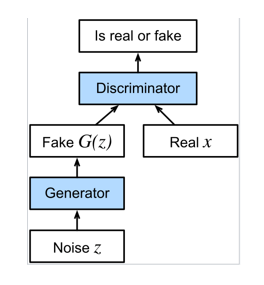
\includegraphics[width=0.5\textwidth]{Imgs/GAN_General_Arch.png}
    \caption{GAN General Architecture}
    \label{fig:GAN_Arch}
\end{figure}



\subsubsection{\ac{SDA}} \ac{SDA} is a deep neural network architecture designed for unsupervised feature learning and robust data representation\cite{vincent2010sda}. It is constructed by stacking multiple denoising autoencoders on top of each other, where each autoencoder layer is trained to reconstruct its input from a corrupted version of it. The key idea behind an \ac{SDA} is to intentionally introduce noise into the input data and force the network to learn a compressed representation that captures the underlying structure of the data rather than memorizing it. Each individual denoising autoencoder consists of an encoder function that maps the input vector to a latent representation and a decoder function that attempts to reconstruct the original clean input. After training one layer, its encoded output is used as the input to the next layer, allowing the network to progressively learn higher-level and more abstract features. This layer-wise training strategy improves convergence and helps mitigate issues such as vanishing gradients in deeper architectures. In anomaly detection scenarios, such as in \ac{ICS}, a \ac{SDA} is typically trained only on benign (normal) data so that it learns a faithful representation of normal system behavior.

\section{Provided Datasets}

For our project we were presented with two different datasets.
Electra\footnote{\url{http://perception.inf.um.es/ICS-datasets/csv/electra_s7comm.zip}} and 2017QUTS7Comm \footnote{ \url{https://github.com/qut-infosec/2017QUT_S7comm}} 
The Electra S7Comm dataset and the 2017QUTS7Comm dataset differ substantially in origin, structure, and format. Electra S7Comm was published by the University of Murcia (Spain) and was collected from realistic industrial testbeds~\cite{electra}. In contrast, 2017QUTS7Comm was generated in a controlled laboratory environment by the Queensland University of Technology~\cite{acisp2017}.



\subsection{Statistical Characteristics}
The Electra S7Comm dataset comprises approximately 387 million packets,
with roughly two thirds benign traffic and one third attack traffic.
All packets belong to the S7Comm protocol over \ac{TCP}.
Communication is limited to four host pairs, consisting of two benign
communication pairs and two attack-related pairs.

The 2017QUTS7Comm dataset contains approximately 10.8 million packets
and exhibits a strong class imbalance toward attack traffic.
While S7Comm constitutes the majority of traffic, additional
application-layer protocols such as \ac{NTP}, DHCPv6, \ac{NBNS}, and \ac{mDNS} are present.
Both \ac{TCP} and \ac{UDP} transport protocols occur in the dataset.

In total, 26 distinct host communication pairs are observed in
2017QUTS7Comm. However, the attack traffic is generated from a limited
set of attacker endpoints, with attack activity primarily originating
from a single source IP address interacting with different targets.
